% !TeX spellcheck = en_US
\chapter{GraphRePair vs HDT}\label{ch:GRPvsHDT}

This chapter deals with the comparison between HDT and GRP. The main aim is to determine which of the two compressors achieves a lower compression ratio.

In Ch.~\ref{sec:theory} some basic concepts of the compressors will be discussed again and hypotheses will be made how the compression rate behaves in relation to a certain structuring of RDF data. 

In Ch.~\ref{sec:data_creation} it will be considered how data can be generated that is structured in the way stated in Ch.~\ref{sec:theory}.

Finally in Ch.~\ref{sec:evalHDT} an empirical evaluation of the compression ratios for HDT and GRP for that synthetic RDF data will be done. The evaluation will show that the hypotheses stated in Ch.~\ref{sec:theory} are correct.

\section{Theory}\label{sec:theory}
The obvious question is now whether there are certain properties/features that an RDF graph can have, and which have a positive or negative impact on the compression ratio of one or both algorithms. 

\subsection{Relation between data structure and compression ratio}

First these features are considered for HDT. Fig.~\ref{fig:hdt_overview_1} is shown again. There you can see that the size of the data becomes smaller if there are only a few subjects. This is the case because the bit-array $B_p$ contains a 1 every time a new subject is considered. For example, if there is only one subject, then $B_p$ consists only of zeros.

\begin{figure}[h]
	\centering
	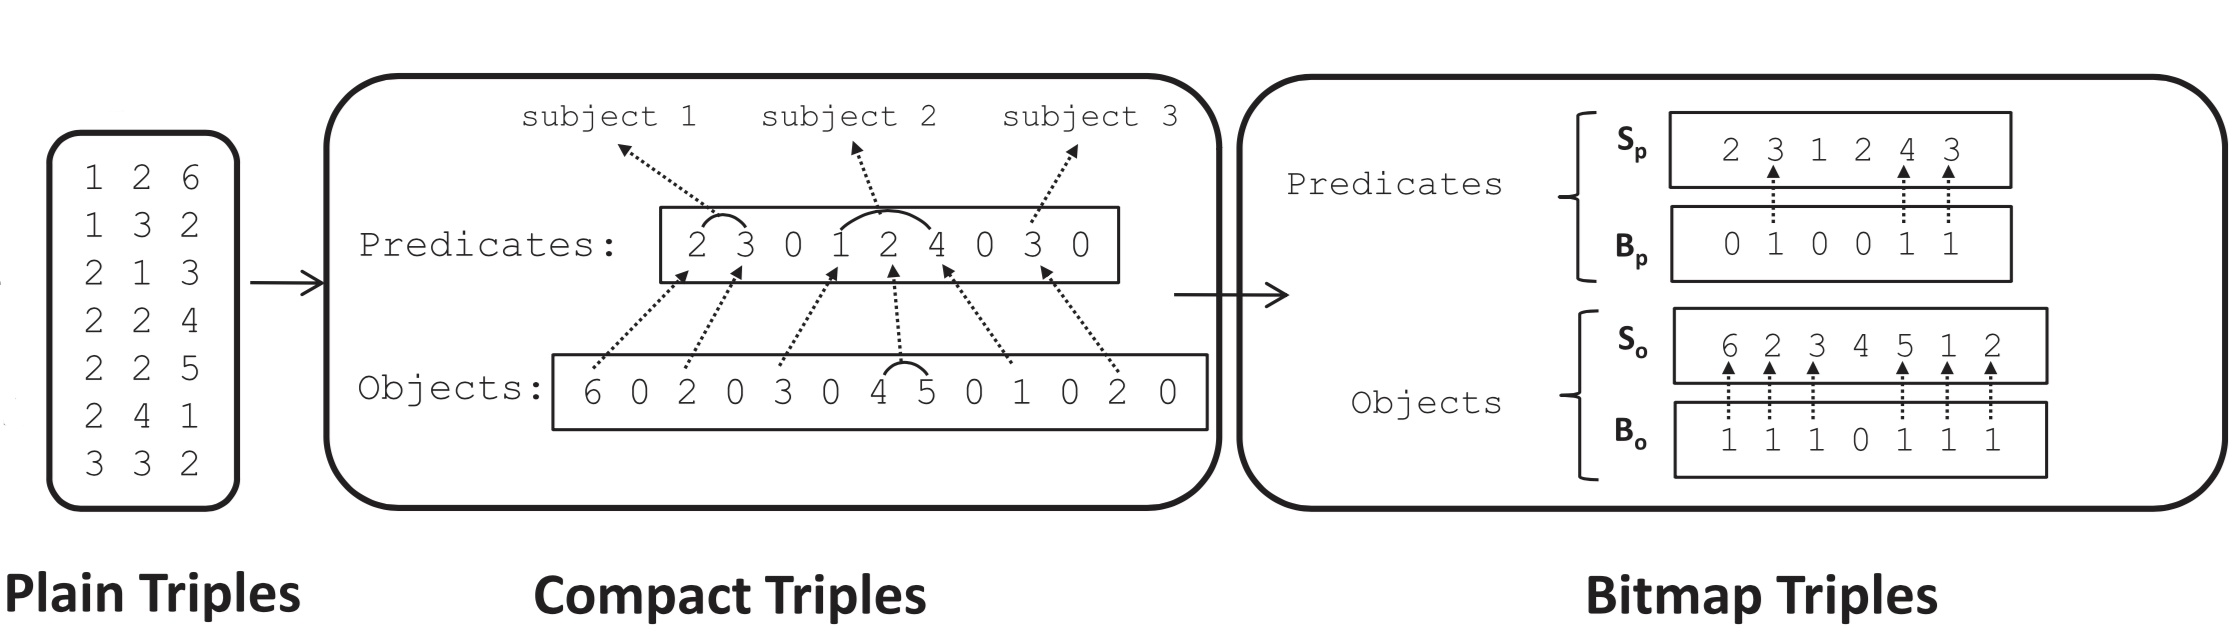
\includegraphics[width=1\textwidth]{figures/relatedwork/hdt1}
	\caption{Three different representations of triples in HDT}
	\label{fig:hdt_overview_1}
\end{figure}

For GRP that feature analysis is more complex. Since GRP constructs grammar rules by using the graph's structure, it is more dependent on the data's structure than HDT. There can be many features that can lead to different constructible grammar rules. Those will not be discussed here. But a simple insight is that GRP's compression ratio will be bigger when there are more different predicates in the graph. This is true, because GRP's grammar rules are based on the repeating edge labels. That fact will be considered in the evaluation.

\subsection{Dictionary Size}

As already explained in Ch.~\ref{ch:related_work}, HDT divides an RDF file into its header, dictionary and triples component. This partially also true for GRP except that GRP does not create a header. But it also assigns an ID to every URI or literal and then only works with these IDs. Unfortunately the authors of~\cite{maneth} did not work on efficient storing of the dictionary. In GRP the size for the dictionary component is just ignored. Therefore we have to add this size in order to compare GRP with HDT in a fair way. To achieve that we just add the same size to the compressed size of GRP that HDT would need to store the dictionary.

\section{Synthetic Data Creation}\label{sec:data_creation}

As has just explained, HDT can compress a graph that is similar to a hub pattern (few subjects, many objects) very well. So it gets worse the further away the graph is from this pattern. This corresponds to the authority pattern, where there are few objects but many subjects.

The task now is to create a series of RDF graphs that first correspond to the hub pattern and then continue to change in the direction of the authority pattern. This is illustrated in Fig.~\ref{fig:star_pattern}. In this scenario all graphs ($G_1$ to $G_m$) have the same size, i.e. the same number of nodes and edges. $G_1$ has only one subject connected to all objects. $G_2$ then has two subjects more and correspondingly 2 objects less. This goes on and on until there is only one object that is connected to all subjects ($G_m$). The edges are randomly distributed among the nodes, so that all nodes have a similar degree and each node has at least a degree of one.

\begin{figure}[h]
	\centering
	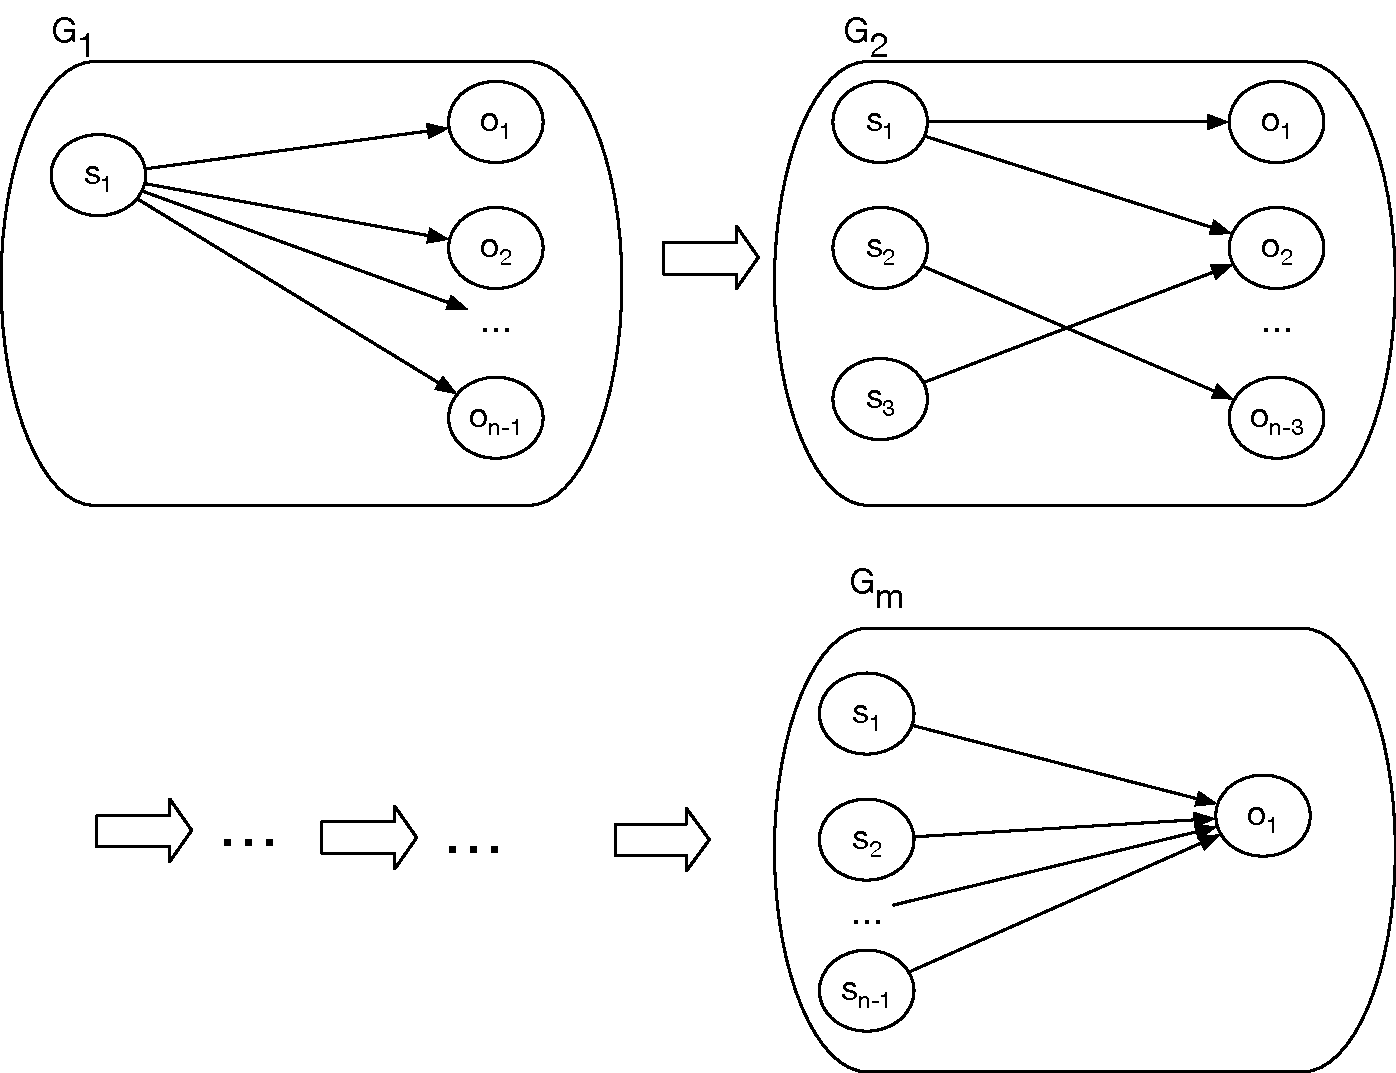
\includegraphics[width=0.8\textwidth]{figures/GRPvsHDT/starpattern.pdf}
	\caption{Step-by-step transition from hub pattern to authority pattern. The number of nodes $n$ is the same for each graph. The number of edges is also the same for each graph.}
	\label{fig:star_pattern}
\end{figure}

It is also ensured that each of the generated files has exactly the same size. This is made possible by ensuring that each URI has the same length. Since the RDF graph also has the same number of triples, the files are of the same size. Since the evaluation compares the compression ratios for the different RDF files, it is important that all files are the same size to ensure a fair comparison.

A section of such a file (for $G1$) is shown in Fig.~\ref{fig:rdfFile}. In this example, there is only one predicate for all triples. The number of predicates is always one at first. The amount of predicates has a similar effect on both compressors and is therefore omitted at first. But in Ch.~\ref{sec:evalHDT} that effect will be discussed in more detail.

Apart from that, blank nodes and literals are not used here. For both compressors, blank nodes and literals are being handled analogously to URI nodes. Therefore they are not needed at this point, in order to show the behavior of HDT and GRP in the above described scenario.

\begin{figure}[h]
	\centering
	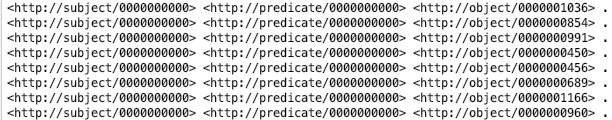
\includegraphics[width=0.8\textwidth]{figures/GRPvsHDT/file.png}
	\caption{Excerpt from the generated RDF file for $G_1$ (see Fig.~\ref{fig:star_pattern}). Each triple has the same length.}
	\label{fig:rdfFile}
\end{figure}

\section{Evaluation}\label{sec:evalHDT}

For the following evaluation HDT-Java 2.0~\footnote{\label{foot:1}https://github.com/rdfhdt/hdt-java/releases/tag/v2.0} (the currently newest version) has been used. For GRP the implementation mentioned in~\cite{maneth} has been used (written in Scala). It is not open source and has been given to us by the authors of~\cite{maneth}.

Fig.~\ref{fig:ratiosHDTWithoutDict} shows the compression ratio for HDT (without dictionary size). As expected, the ratio gets higher the more similar the graph is to the authority pattern. In general it can be said that this effect is quite small. There is only a distance of 0.002 between the minimum and the maximum. This small effect can also be seen by looking at Fig.~\ref{fig:ratiosHDTWithDict}. It can be seen that the size of the dictionary has a much bigger effect, since the compression ratio is now much larger and the curve behavior from Fig.~\ref{fig:ratiosHDTWithoutDict} is no longer recognizable. It is noticeable that the dictionary size gets bigger when the graph is further away from the star pattern. The dictionary implementation of HDT seems to be more inefficient when there are about as many subject as objects. 


\begin{figure}[h]
	\centering
	\subfloat[Without dictionary size.]{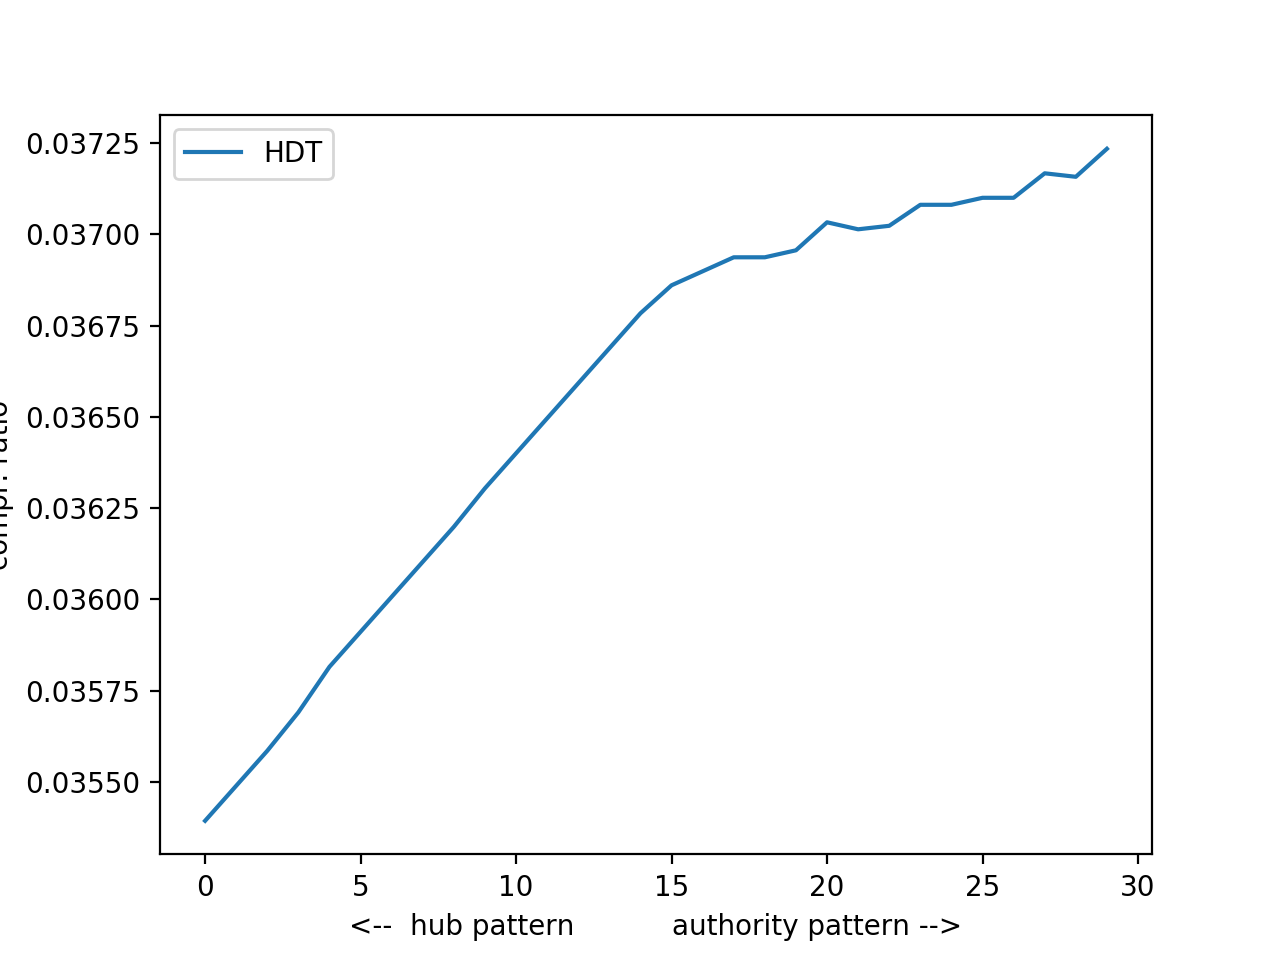
\includegraphics[width=0.5\textwidth]{figures/GRPvsHDT/hdtWithoutDict}\label{fig:ratiosHDTWithoutDict}}
	\hfill
	\subfloat[With dictionary size.]{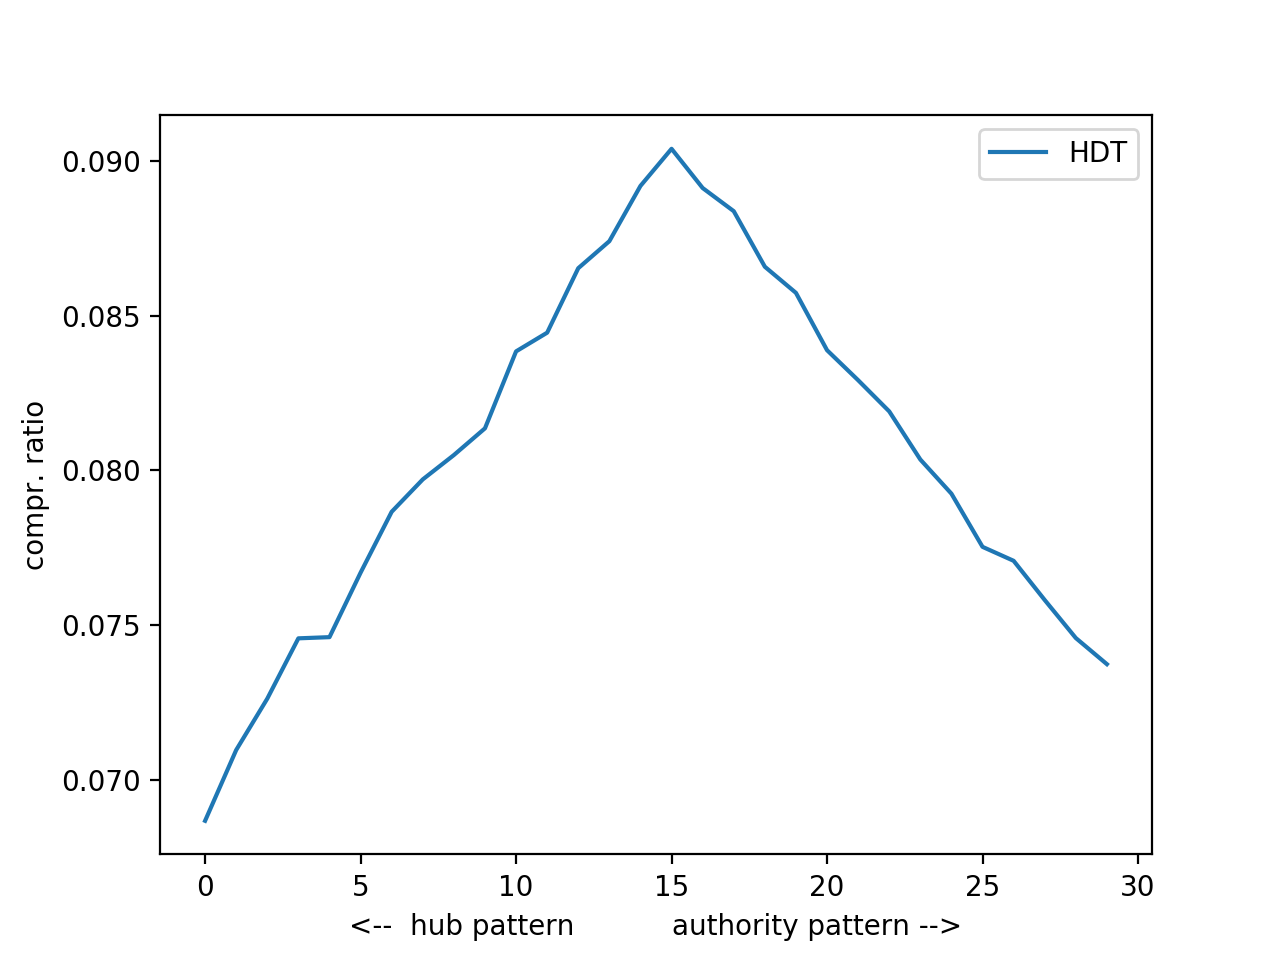
\includegraphics[width=0.5\textwidth]{figures/GRPvsHDT/hdtWithDict}\label{fig:ratiosHDTWithDict}}
	\caption{The compression ratios for HDT without and with dictionary sizes.}
\end{figure}

Next the compression ratio of GRP is considered, which is presented in Fig.~\ref{fig:ratiosGRPWithoutDict} (without dictionary sizes). Here you can see that GRP has a better compression ratio if the graph is more similar to the star pattern (hub order authority pattern). This property of GRP has also been mentioned in~\cite{maneth}. It can also be seen that the effect on the compression ratio is bigger for GRP than for HDT (standard deviation is twice as high for GRP as for HDT). A grammar-based compression is therefore more dependent on the structure of the input data.

When Fig.~\ref{fig:ratiosGRPWithDict} is considered, it can be seen that this curve behaves almost exactly like the one from Fig.~\ref{fig:ratiosHDTWithDict}, since the size of the dictionary accounts for most of the compressed data size.

\begin{figure}[h]
	\centering
	\subfloat[Without dictionary size.]{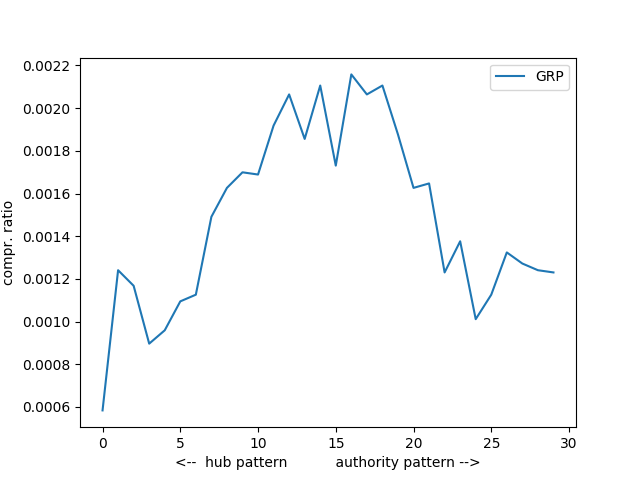
\includegraphics[width=0.5\textwidth]{figures/GRPvsHDT/grpWithoutDict}\label{fig:ratiosGRPWithoutDict}}
	\hfill
	\subfloat[With dictionary size.]{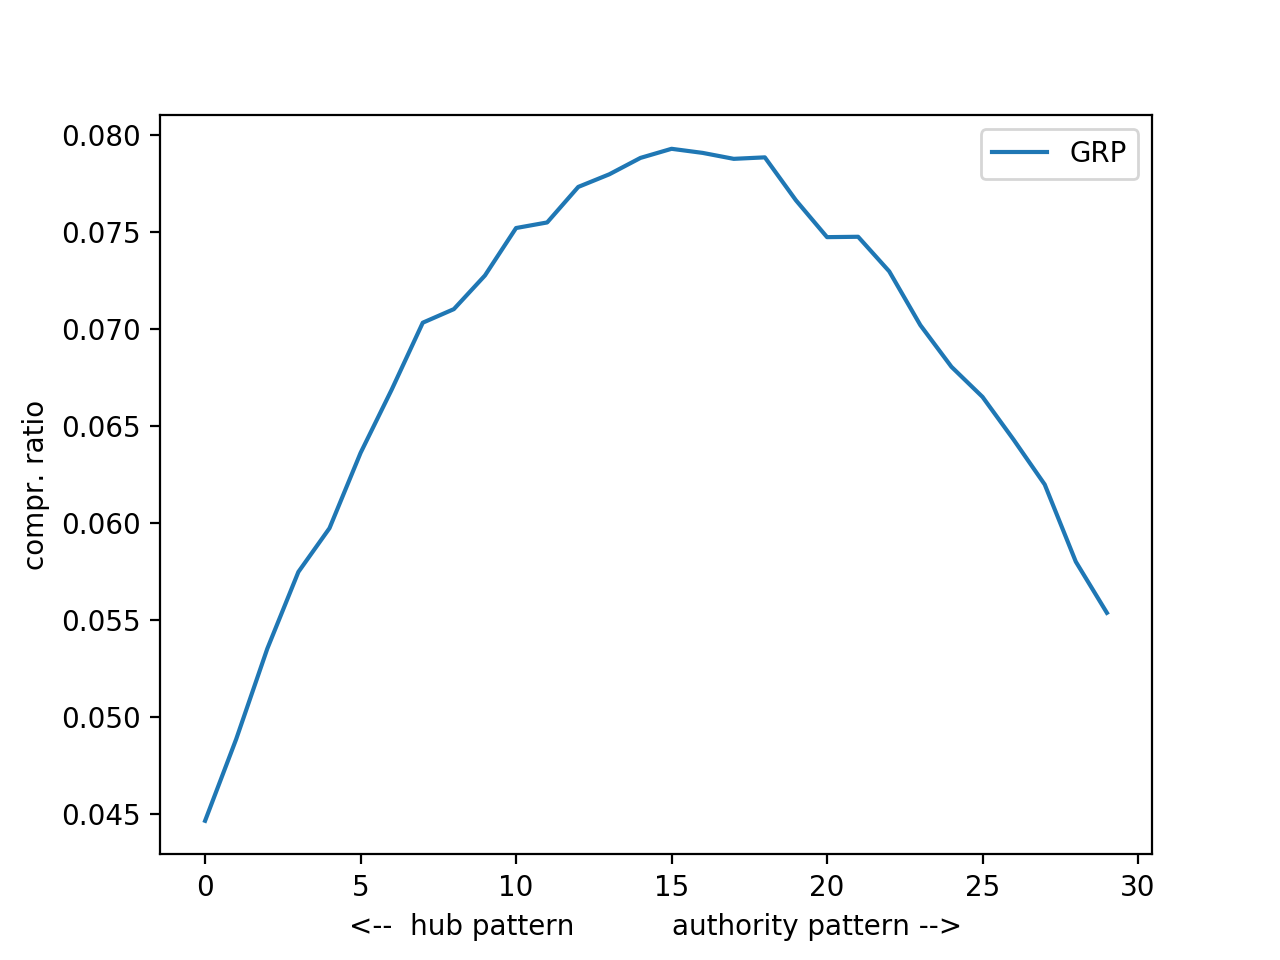
\includegraphics[width=0.5\textwidth]{figures/GRPvsHDT/grpWithDict}\label{fig:ratiosGRPWithDict}}
	\caption{The compression ratios for GRP without and with dictionary sizes.}
\end{figure}

Finally, Fig.~\ref{fig:ratiosBothWithoutDict} and Fig.\ref{fig:ratiosBothWithDict} show the compression ratios for both algorithms. Since both use the same method to compress the dictionary, the curves in Fig.~\ref{fig:ratiosBothWithDict} are very similar. However, it becomes clear that GRP compresses better than HDT. In Fig.~\ref{fig:ratiosBothWithoutDict}, the ratio of HDT is 31 times higher on average. Of course, this factor becomes much smaller in Fig.~\ref{fig:ratiosBothWithDict} because the dictionary accounts for most of the memory size. Here the compression ratio of HDT is on average 1.8 times as high as that of GRP.

\begin{figure}[h]
	\centering
	\subfloat[Without dictionary size.]{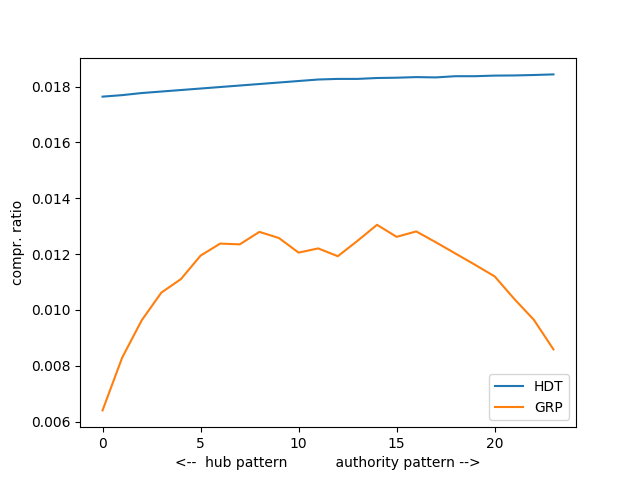
\includegraphics[width=0.5\textwidth]{figures/GRPvsHDT/bothWithoutDict}\label{fig:ratiosBothWithoutDict}}
	\hfill
	\subfloat[With dictionary size.]{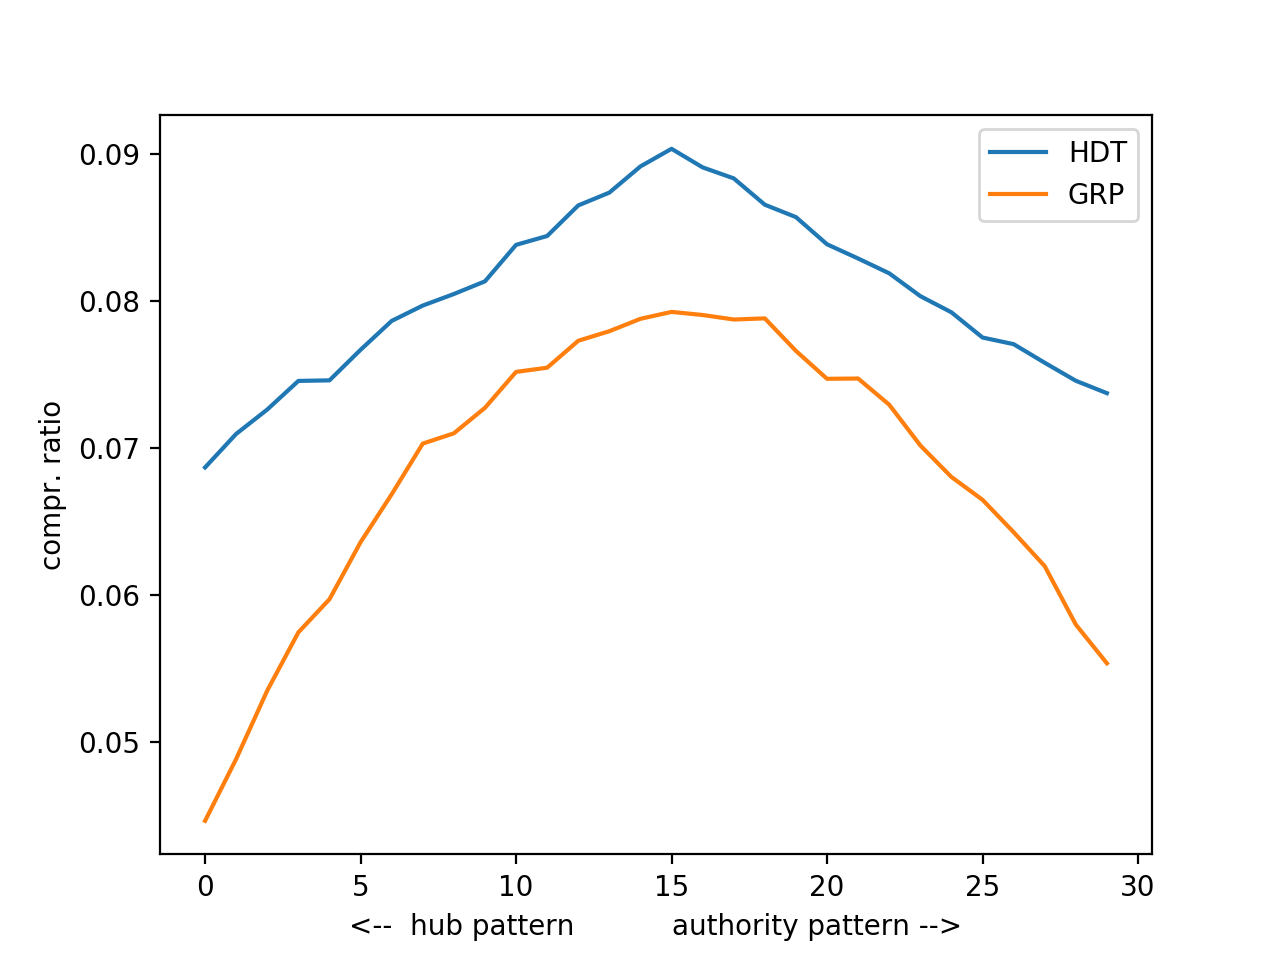
\includegraphics[width=0.5\textwidth]{figures/GRPvsHDT/bothWithDict}\label{fig:ratiosBothWithDict}}
	\caption{The compression ratios for GRP and HDT without and with dictionary sizes.}
\end{figure}

One could now argue that only one distinct predicate was used in that scenario and this is beneficial for GRP, as it gets worse as the number of predicates increases. Therefore a further evaluation is made in Fig.~\ref{fig:bothwithdict1000predicates}, where 1000 distinct predicates have been used. That is a quite high number considering the number of triples (1199) compared to real RDF data \todo{belegen}. One can see that the compression ratios are now higher for both compressors, but still GRP's ratio is always smaller than HDT's. HDT's ratio is still 1.7 times higher on average. So, the increasing number of predicates has a similar effect on both algorithms.

\begin{figure}
	\centering
	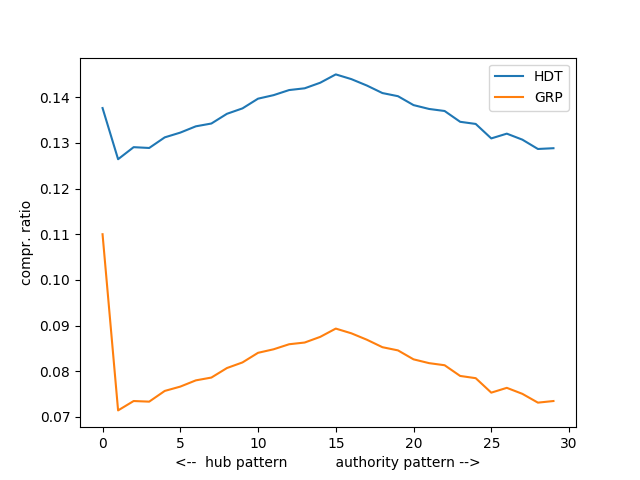
\includegraphics[width=0.7\linewidth]{figures/GRPvsHDT/bothWithDict1000Predicates}
	\caption{The compression ratios for GRP and HDT with dictionary sizes. Graphs have now 1000 distinct predicates.}
	\label{fig:bothwithdict1000predicates}
\end{figure}

Apart from the compression ratio, the run time is also important for the overall performance. Fig.~\ref{fig:runtimes} shows the average run times of the two algorithms. For this the same scenario with the star pattern (and only one distinct predicate) was used. It has been executed 100 times to get a sophisticated run time measurement, because the run time also depends on the current CPU workload of the computer.

\begin{figure}
	\centering
	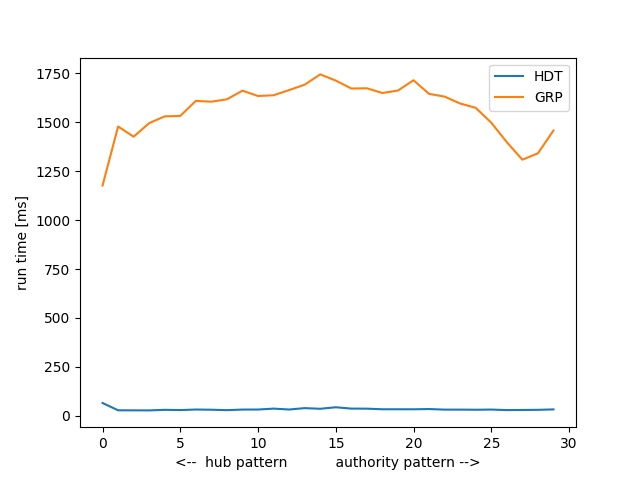
\includegraphics[width=0.7\linewidth]{figures/GRPvsHDT/runtimes}
	\caption{Run times of both algorithms (average run time of 100 consecutive executions).}
	\label{fig:runtimes}
\end{figure}


It can be seen that the runtime of GRP is significantly higher than that of GRP. It is on average ca. 48 times as high.

However, it should also be noted that the implementation of GRP is rather rudimentary  (according to the authors of~\cite{maneth}), while that of HDT has been under development for some time. So they are not comparable in terms of quality. Unfortunately, one cannot say at this point whether a more professional implementation of GRP will also be slower than HDT.

In addition one can notice that GRP's run time fluctuates more than that of HDT. GRP has a standard deviation of about 134, while HDT only has a standard deviation of about 7. One reason for this is that GRP, in contrast to HDT, is non-deterministic because of the partly random search order of the graph. On the other hand, the high deviations are also a confirmation of the above mentioned hypothesis that the behavior of GRP depends more on the structure of the input data than HDT does.























